\documentclass{article}
\usepackage[utf8]{inputenc}
\usepackage{amssymb}
\usepackage{amsmath}
\addtolength{\oddsidemargin}{-.875in}
\addtolength{\evensidemargin}{-.875in}
\addtolength{\textwidth}{1.75in}

\addtolength{\topmargin}{-1in}
\addtolength{\textheight}{1.75in}

\usepackage{graphicx}
\graphicspath{ {./Desktop/Notes/MA106} }

\title{MA106}
\author{Shubh Kumar}
\date{IIT-B, Spring Semester 2021}

\begin{document}

\maketitle

\section{Lecture 1: Introduction}
\begin{itemize}
    \item Matrices are a new universe of Numbers
    \item Visualizing the matrices as a column vector of row vectors or a row vector of column vectors, is an important thing
    \item Outer Product is called so, as its sort of doing the inner product/scalar product(or dot product!), the other way round!
    \item Going over the various ways to write the Product of Two Matrices

    \item Exercise: Proving Trivial Results like $\big(\textbf{AB}\big)^T$ = $\mathbf{B^{T}}$ $\mathbf{A^{T}}$

    \item The $j^{th}$ row of \textbf{AB} is a linear combination of the $j^{th}$ row of \textbf{A} with coefficient of some common, and analogically in case of $k^{th}$ column of \textbf{AB} would be
    \item Really Nice Question: Justifying the different cases of solutions to system of linear equations using concepts from matrices
\end{itemize}

\section{Lecture 2: Linear Systems}

\begin{itemize}
    \item General Linear system will include homogeneous as well as non-homogeneous.
    \item \textbf{Deducing Connections:} How to relate $\mathbf{Ax = b}$ to $\mathbf{Ax = 0}$. If $\mathbf{Ax = 0}$ has non-trivial solutions, than that would mean infinitely many solutions if we know just one solution exists.

    \item Extending the past concepts to more general cases: Using the above thing to solve any general system of m equations in n variables.

\end{itemize}

\section{Lecture 3: Gaussian Elimation}
Nothing as such apart from Lecture Notes introduced,
Just a very nice and thoughtful question:
Let $\mathbf{A} \in \mathbb{R}^{9x4}$ and $\mathbf{B} \in \mathbb{R}^{7x3}$. Is there $\mathbf{X}
\in \mathbb{R}^{4x7}$ such that $\mathbf{X} \ne \mathbf{O}$ but $\mathbf{AXB = O}$

\section{In General Observations/Queries which people posted on Whatsapp Group}
\begin{itemize}
  \item From LEC2, where first we identify the pivot points in REF, identify the free and non-free variables
  and then set the non-free ones to zero, following which we also identify the basis vectors by setting each one of
  them to one in and getting separate solutions, so that the overall solution is a linear combination of these.

  \item In the REF of an inconsistent System, we can get different REFs there is no unique one, but we do have
  a unique Reduced REF or Row-canonical Form.

  \item Another way to progress, after we've identified the Free variables in REF, would be to simply substitute
  the Free variables $x_i = \alpha_i$, but we don't do this, Why?

  \item 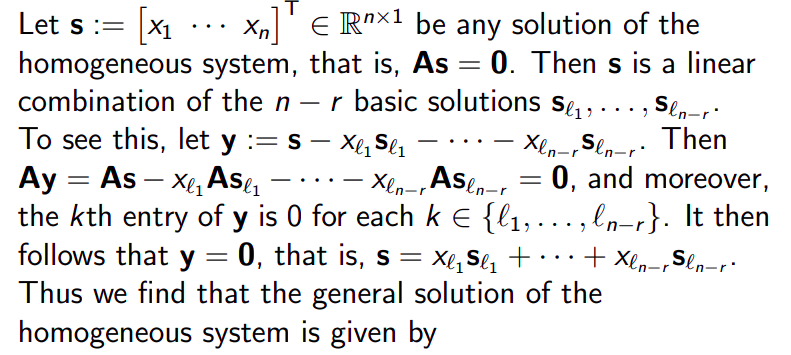
\includegraphics[scale = 0.5]{1.png} \\ Why is $\mathbf{y} = 0$ in the above paragraph?
  \item Try proving: For all $\mathbf{A} \in \mathbb{R}^{nxn}$ if  $\mathbf{AE=EA}$, for some $\mathbf{E} \in \mathbb{R}^{nxn}$
  such that $\mathbf{E = I}$.
  \item Let $I \subset \mathbb{R}^{n × n}$ be a nonempty set closed under addition such that $\mathbf{MN, NM} \in I $ whenever $\mathbf{N} \in I$ and $\mathbf{M} \in \mathbb{R}^{nxn}$. Show that either $I = 0$ or $I = \mathbb{R}^{nxn}$.
  \item

\end{itemize}
\end{document}
